% Artigo do Lab03 -- Mineração de Métricas DORA.
%
% O sbc-template.sty e o sbc.bst são os do modelo oficial da SBC
% (https://www.sbc.org.br/documentosinstitucionais/#publicacoes). Para compilar, nesta pasta:
%
%   pdflatex artigo && bibtex artigo && pdflatex artigo && pdflatex artigo
%
% As seções vêm dos .tex de ../docs/, que são a versão condensada do artigo (máximo de 10
% páginas); os .md de lá são a versão estendida, com mais detalhes. As figuras vêm de
% ../resultados/, geradas pelos scripts de ../analises/.
%

\documentclass[12pt]{article}

\usepackage{sbc-template}
\usepackage{graphicx,url,amsmath}
\usepackage[utf8]{inputenc}
\usepackage[T1]{fontenc}
\usepackage[brazilian]{babel}

\graphicspath{{../resultados/}}
\sloppy

\title{Métricas DORA em projetos open-source: o que se pode medir com dados públicos do
GitHub}

\author{João Santana Lopes\inst{1}, Pedro Maia\inst{1}, Arthur Candian\inst{1}}

\address{Pontifícia Universidade Católica de Minas Gerais (PUC Minas)\\
  Laboratório de Experimentação de Software
  \email{joaovslopes20@gmail.com, pedromaiasilva17@gmail.com,}\\ \footnotesize\texttt{acandian15@gmail.com}
}

\begin{document}

\maketitle

\begin{abstract}
The DORA metrics describe software delivery performance through four indicators, but they
were established from self-reported surveys of corporate teams, which makes them neither
auditable nor obviously applicable to open-source projects. We compute the four metrics for
350 popular GitHub repositories over a fixed 12-month window, using only public API data,
with releases as a proxy for deployments and failed CI runs as a proxy for failed changes. We
validate the proxies against a gold sample of 60 repositories and 299 releases labelled
independently by three raters. The median deployment frequency is 0.42 releases per week and
the median recovery time is 2.56 hours, but the change failure rate depends critically on how
failure is operationalised: the CI proxy and the delivery proxy correlate at only
$\rho = 0.107$ and disagree on the DORA category of 20.6\% of the sample. A sensitivity
analysis over three definitions of deployment moves between 25\% and 33\% of repositories
across categories. We conclude that DORA classifications derived from public repository data
are contingent on operational choices that are rarely made explicit.
\end{abstract}

\begin{resumo}
As métricas DORA descrevem o desempenho de entrega de software por quatro indicadores, mas
foram estabelecidas a partir de questionários autorrelatados por equipes corporativas, o que
as torna não auditáveis e de aplicação incerta a projetos \textit{open-source}. Calculamos as
quatro métricas para 350 repositórios populares do GitHub em uma janela fixa de 12 meses,
usando apenas dados públicos da API, com \textit{releases} como \textit{proxy} de
\textit{deploy} e falhas de CI como \textit{proxy} de falha. Validamos os \textit{proxies}
contra uma amostra-ouro de 60 repositórios e 299 \textit{releases}, rotuladas de forma
independente por três avaliadores. A mediana da frequência de \textit{deploy} é de 0,42
\textit{release} por semana e a do tempo de recuperação é de 2,56 horas, mas a taxa de falha
depende de como a falha é operacionalizada: o \textit{proxy} de CI e o de entrega
correlacionam-se a apenas $\rho = 0{,}107$ e discordam sobre a categoria DORA de 20,6\% da
amostra. Uma análise de sensibilidade sobre três definições de \textit{deploy} move entre
25\% e 33\% dos repositórios de categoria. Concluímos que classificações DORA obtidas de
dados públicos são contingentes a escolhas operacionais raramente explicitadas.
\end{resumo}

% ---------------------------------------------------------------- Introdução
\section{Introdução}

% Introdução (seção escrita pelos três).
% As hipóteses entram logo depois, de hipoteses_rq3_rq5.tex.

As métricas DORA, propostas pelo programa \textit{DevOps Research and
Assessment}~\cite{dora2024}, descrevem o desempenho de entrega de uma equipe por quatro
indicadores: frequência de \textit{deploy}, \textit{lead time} para mudanças, taxa de falha
das mudanças (CFR) e tempo de recuperação. Com os quatro, a equipe é classificada como
\textit{Elite}, \textit{High}, \textit{Medium} ou \textit{Low}, e a literatura associa as
categorias superiores a práticas como integração contínua e implantação em pequenos
lotes~\cite{forsgren2018}. As faixas vieram de questionários autorrelatados por equipes
corporativas, que não podem ser auditados, e não se sabe o que significam em projetos
\textit{open-source}, cujo ritmo de publicação é decidido por mantenedores voluntários.

Neste trabalho calculamos as quatro métricas apenas com dados públicos do GitHub, para 350
repositórios populares que usam GitHub Actions, em uma janela fixa de 12 meses. Como a API
não informa quando uma mudança chegou à produção nem quando um defeito afetou usuários,
usamos dois \textit{proxies}: a publicação de uma \textit{release} aproxima o
\textit{deploy}, e a falha de um \textit{workflow} de CI aproxima a falha de uma mudança.
Também verificamos esses \textit{proxies}: três avaliadores rotularam uma amostra-ouro de 60
repositórios e 299 \textit{releases}, contra a qual avaliamos a heurística que identifica
\textit{releases} corretivas, e comparamos três definições de \textit{deploy} para ver o
quanto as conclusões mudam com elas.

\subsection{Questões de pesquisa}

\begin{description}\itemsep0pt
\item[RQ 01] Com que frequência são feitos \textit{deploys} nesses projetos?
\item[RQ 02] Qual o \textit{lead time} para mudanças, nas variantes (a) e (b)?
\item[RQ 03] Qual a taxa de falha das mudanças, nas variantes (a) e (b)?
\item[RQ 04] Qual o tempo de recuperação após uma falha?
\item[RQ 05] Frequência de \textit{deploy} e taxa de falha se correlacionam?
\item[RQ 06] Que características dos repositórios se associam ao desempenho?
\item[RQ 07] A classificação muda se o \textit{deploy} for definido de outra forma?
\item[RQ 08] Qual a proporção de \textit{releases} corretivas (\textit{rework rate})?
\end{description}

A Seção~2 descreve a metodologia, a Seção~3 os resultados, a Seção~4 a discussão, a Seção~5
as ameaças à validade~\cite{wohlin2012} e a Seção~6 as conclusões.


\subsection{Hipóteses}

% Hipóteses informais, uma por RQ (subseção da Introdução).

A Tabela~\ref{tab:hipoteses}, na Discussão, confronta cada hipótese com o que foi observado.

\textbf{RQ 01.} A maioria dos projetos deve publicar menos de uma \textit{release} por semana,
com mediana entre uma por mês e uma por semana (faixa \textit{Medium}), já que
\textit{releases} open-source costumam agrupar várias mudanças.

\textbf{RQ 02.} O \textit{lead time} deve ser de semanas (mediana entre uma semana e 30 dias),
com a variante (a) maior que a (b), porque ela mede a partir do \textit{commit} mais antigo
de cada \textit{release}.

\textbf{RQ 03.} CFR (a) entre 10\% e 25\% na mediana, porque testes instáveis e dependências
externas falham mesmo depois do \textit{pull request}; CFR (b) parecido ou menor, com muitos
zeros; e pouca concordância entre as variantes, que medem falha de \textit{pipeline} e falha
percebida pelo usuário.

\textbf{RQ 04.} Mediana de algumas horas, maioria \textit{High}, cauda longa (mantenedores
trabalham de forma voluntária e assíncrona) e uma proporção não trivial de episódios
censurados.

\textbf{RQ 05.} Correlação fraca negativa ou nula com o CFR (a), como afirma o DORA, e
positiva com o CFR (b), em parte por artefato: quem publica muito tem mais chance de publicar
um \textit{patch} em até 7 dias após qualquer \textit{release}.

\textbf{RQ 06.} Projetos mais populares e com mais contribuidores devem ter desempenho melhor
(publicar mais e com \textit{lead time} menor), projetos mais antigos devem publicar menos,
com ritmo mais estável, e a linguagem deve ter pouco efeito.

\textbf{RQ 07.} A classificação deve ser razoavelmente robusta, com menos de 20\% dos
repositórios mudando de categoria, porque pré-\textit{releases} e \textit{tags} costumam
acompanhar as \textit{releases}; usar \textit{tags} deve aumentar a frequência e o número de
repositórios \textit{Elite}.

\textbf{RQ 08.} O \textit{rework rate} deve ser maior que o CFR (b), por contar toda
\textit{release} corretiva, e ficar em torno de um terço das \textit{releases}.


% ---------------------------------------------------------------- Metodologia
\section{Metodologia}

% Metodologia -- fonte de dados, janela e seleção da amostra (parte do João).
% Vem antes das definições operacionais (Arthur) e da validação manual (Pedro).
% Números de dados/funil.csv, dados/repositorios.csv e do log da coleta.

\subsection{Fonte de dados e coleta}

Todos os dados vêm da API REST do GitHub, consultada por um \textit{pipeline} próprio em
Python que usa apenas a biblioteca \texttt{requests}. A coleta inteira é reproduzida por um
único comando. Cada resposta da API é gravada em um \textit{cache} local indexado pelo
\textit{hash} da URL, de modo que uma coleta interrompida continua de onde parou. A execução
final fez 11.989 chamadas à API e reaproveitou 58.459 respostas do \textit{cache}.

A busca de repositórios devolve no máximo 1.000 itens por consulta, e só a faixa de 1.000 a
1.500 estrelas tem 20.493 repositórios. Por isso, dividimos a busca em sete faixas de
estrelas (1.000--1.500, 1.500--2.500, 2.500--4.000, 4.000--7.000, 7.000--12.000,
12.000--25.000 e mais de 25.000). De cada faixa entraram os 1.000 repositórios mais
estrelados, num total de 7.000 candidatos. Os candidatos foram avaliados alternando as
faixas, para que a amostra não saísse inteira da faixa mais popular.

O cliente HTTP respeita a cota da API, esperando o \textit{reset} quando ela acaba, e repete
erros 5xx e falhas de rede com \textit{backoff} exponencial (1, 2, 4, 8 e 16~s), até seis
tentativas. Todas as listagens são paginadas pelo cabeçalho \texttt{Link}. A listagem de
\textit{workflow runs} também devolve no máximo 1.000 resultados, e o seu
\texttt{total\_count} satura em 2.500. Por isso, os \textit{runs} são pedidos mês a mês, e o
mês que passa do teto é dividido ao meio até caber nele.

\subsection{Janela de observação}

A janela tem 12 meses, de 01/10/2025 a 30/09/2026, inclusiva nas duas pontas, e é a mesma
para todos os repositórios. Só entram releases publicadas e \textit{workflow runs} criados
dentro dela, e só no \textit{default branch}. A idade do repositório é medida até o fim da
janela, e não até a data da execução, para que uma nova execução chegue ao mesmo valor.

\subsection{Seleção da amostra}

Os candidatos passaram por filtros em sequência. Cada repositório parou no primeiro filtro em
que falhou, e por isso tem um único motivo de descarte. A coleta parou ao completar 350
repositórios aprovados, acima do mínimo de 300. A Tabela~\ref{tab:funil} mostra o funil.

\begin{table}[ht]
\centering
\caption{Funil de seleção da amostra.}
\label{tab:funil}
\small
\begin{tabular}{lrrl}
\hline
\textbf{Etapa} & \textbf{Restantes} & \textbf{Descart.} & \textbf{Motivo do descarte} \\
\hline
Candidatos da busca (7 faixas) & 7.000 & -- & -- \\
Avaliados                      & 1.565 & 5.435 & não avaliados (amostra completa) \\
Usam GitHub Actions            & 1.057 & 508 & nenhum workflow \\
$\geq$ 5 releases na janela    & 439   & 618 & menos de 5 releases \\
\textit{Runs} mensuráveis      & 433   & 6   & $>$ 1.000 \textit{runs} em um dia \\
$\geq$ 50 \textit{runs} válidos & 352  & 81  & menos de 50 \textit{runs} válidos \\
Coleta sem erro                & 350   & 2   & erro definitivo da API \\
\hline
\textbf{Amostra final}         & \textbf{350} & -- & -- \\
\hline
\end{tabular}
\end{table}

Os 5.435 candidatos não avaliados nunca foram consultados, porque a coleta parou ao fechar
a amostra; eles não foram reprovados por critério algum. Os seis repositórios com mais de
1.000 \textit{runs} em um único dia foram descartados porque não há como recuperar todos os
\textit{runs} desses dias, nem saber quantos faltam. Mantê-los faria o CFR~(a) e o tempo de
recuperação serem calculados sobre dados truncados. Com isso, a amostra exclui os projetos de
maior volume de CI. Os dois erros definitivos foram um HTTP 504 recorrente e uma listagem de
releases que passou do limite de 10.000 resultados paginados da API.

A amostra final reúne 350 repositórios com 1.493 a 291.317 estrelas (mediana de 11.944),
concentrados nas faixas mais populares: 97 têm mais de 25.000 estrelas e 27 estão na faixa
de 1.000 a 1.500. As linguagens mais frequentes são TypeScript (73), Python (72), Go (45),
Rust (39) e JavaScript (28). A mediana é de 22 releases e 688 \textit{runs} válidos por
repositório na janela, e a idade mediana é de 6,0 anos.

A amostra não é aleatória. Dentro de cada faixa, só os 1.000 repositórios mais estrelados
chegaram a ser candidatos. Além disso, as faixas foram avaliadas na mesma proporção, mas os
repositórios mais populares passaram mais nos filtros, e por isso a amostra final pende para
eles. Os resultados valem para repositórios populares que usam GitHub Actions e publicam
releases, e não para o GitHub como um todo.

\subsection{Dicionário de dados}

O \textit{pipeline} gera dois arquivos. O \texttt{repositorios.csv} tem uma linha por
repositório avaliado, aprovado ou descartado, e o \texttt{funil.csv} tem uma linha por etapa
da seleção. O dicionário completo, com tipo, unidade e origem de cada coluna, está no
repositório do trabalho. As colunas de \texttt{repositorios.csv} formam cinco grupos:
(i) metadados (estrelas, linguagem, \textit{default branch}, idade e contribuidores);
(ii) contagens da seleção (releases na janela, sem rascunhos e pré-releases, e
\textit{runs} válidos, isto é, de \texttt{push} no \textit{default branch} que terminam em
sucesso ou falha); (iii) as métricas DORA em todas as variantes, com as contagens da
heurística de release corretiva e a proporção de episódios censurados; (iv) a nota de 1 a 4
por métrica e a categoria geral; e (v) o motivo do descarte. Valor vazio significa
\textit{não medido}, e não zero; métrica vazia não recebe nota e fica fora da mediana da
categoria geral.

% Rascunho da parte do Artur na Metodologia (template SBC).
% Trechos [[ ]] dependem da validação manual.

\subsection{Definições operacionais}

Como o GitHub não registra \textit{deploys} nem falhas em produção, todas as métricas são
medidas por \textit{proxies}. Consideramos \textit{deploy} uma release publicada
(\texttt{draft = false}) no \textit{default branch}; pré-releases e tags entram apenas como
variantes na análise de sensibilidade. A frequência de deploy é o número de releases na
janela dividido pelo número de semanas da janela.

O \textit{lead time} é calculado em duas variantes a partir de \texttt{compare/\{anterior\}...\{R\}}
e de \texttt{commit.author.date}: (a) por release, pela diferença entre a data da release e a
do commit mais antigo incluído; (b) por commit, sobre todos os commits de todas as releases.
Releases sem release anterior ou com \texttt{compare} em 404 são ignoradas e contabilizadas.

A \textit{change failure rate} (CFR) também tem duas variantes: (a) a proporção de execuções
de CI com falha, que mede falha de \textit{pipeline} e não de produção; (b) a proporção de
releases seguidas de uma release corretiva em até 7 dias.

\subsection{CFR (b): proxy de entrega}

Uma release R é considerada falha se for seguida, em até 7 dias, por uma release corretiva.
O CFR (b) é o número de releases que falharam dividido pelo número de releases avaliadas.
Releases publicadas nos últimos 7 dias da janela não podem ser avaliadas e ficam fora do
denominador (censura), sendo reportadas.

Como o GitHub não indica se uma release é corretiva, usamos uma heurística sobre a versão
(SemVer) e o assunto dos commits entre as duas releases. R é comparada apenas com a release
seguinte; lemos só o assunto do commit; quando o \texttt{compare} falha, vale apenas o critério
de versão; a primeira release do repositório nunca é corretiva. Testamos três versões:
v1 (só \textit{patch} ou algum commit \texttt{fix}/\texttt{revert}/\texttt{hotfix}), v2 (só
\textit{patch} ou ao menos metade dos commits são correções) e v3 (\textit{patch} com algum
commit de correção, ou ao menos metade dos commits são correções).

\subsection{Validação da heurística}

Sorteamos 60 repositórios da amostra final (\texttt{random\_state = 42}) e 5 releases de cada
um. Os três integrantes rotularam as releases de forma independente, sem ver a saída da
heurística, e o consenso seguiu o protocolo da seção de validação manual. Comparamos a
heurística com o consenso por precisão, recall e F1 da classe ``corretiva'', aceitando
F1 $\geq$ 0,70.

[[ Tabela com v1, v2 e v3 e a versão escolhida ]]

% Metodologia -- protocolo de validação manual (parte do Pedro).

\subsection{Validação manual}

Sorteamos 60 repositórios da amostra (\texttt{df.sample(n=60, random\_state=42)}, após
ordená-los pelo nome) e, de cada um, 5 \textit{releases} com \textit{release} anterior e
\texttt{compare} disponível; um repositório tinha só 4, e a amostra ficou com 299. Os três
autores rotularam de forma independente, sem consultar uns aos outros nem a saída da
heurística: (i) o tipo do projeto (biblioteca, aplicação, CLI ou outro); (ii) se as
\textit{releases} representam entregas reais ao usuário; e (iii) se cada \textit{release} é
corretiva, lendo as \textit{release notes} e os \textit{commits}. Medimos a concordância pelo
kappa de Fleiss, interpretado pela escala de Landis e Koch~\cite{landis1977}
(Tabela~\ref{tab:kappa}). O consenso é a maioria simples; empates 1-1-1 iriam para reunião,
mas não houve nenhum.

\begin{table}[ht]
\centering
\caption{Concordância entre os três avaliadores na amostra-ouro.}
\label{tab:kappa}
\small
\begin{tabular}{lcccc}
\hline
\textbf{Dimensão} & \textbf{Itens} & \textbf{Divergências} & \textbf{$\kappa$} & \textbf{Concordância} \\
\hline
Tipo do projeto             & 60  & 9  & 0,835 & Quase perfeita \\
Releases são entregas reais & 60  & 1  & 0,745 & Substancial \\
Release corretiva           & 299 & 26 & 0,876 & Quase perfeita \\
\hline
\end{tabular}
\end{table}

O menor kappa, o de entregas reais, vem do desbalanceamento: o consenso pôs 59 dos 60
repositórios em ``sim'', e com isso uma única divergência derruba o coeficiente, embora a
concordância bruta seja de 98,3\%. O tipo do projeto teve mais divergências, em projetos que
entregam ao mesmo tempo um servidor e um SDK e no alcance da categoria ``outro''. Em
\textit{release} corretiva, as 26 divergências vêm de \textit{releases} que misturam correções
e novidades. Como a heurística é avaliada contra esse consenso, o kappa de 0,876 serve de teto
prático para ela.


% ---------------------------------------------------------------- Resultados
\section{Resultados}

% Resultados -- RQ 01 a RQ 04 (parte do João).
% Números de resultados/rq1_rq4_*.csv (python -m analises.rq1_rq4_descritiva) e dos
% intervalos de resultados/ic_bootstrap.csv (python -m analises.ic_bootstrap).

Como as distribuições são assimétricas e têm cauda longa, reportamos mediana e IQR. Para
saber o quanto cada número é estável, calculamos também intervalos de confiança de 95\% por
\textit{bootstrap} percentil (2.000 reamostragens dos repositórios, semente fixa) para as
medianas, as correlações e as proporções de mudança de categoria
(Tabela~\ref{tab:descritiva}).

\begin{table}[ht]
\centering
\caption{Estatística descritiva das métricas DORA (350 repositórios) e IC 95\% da mediana.}
\label{tab:descritiva}
\footnotesize
\setlength{\tabcolsep}{4pt}
\begin{tabular}{lrrrrrc}
\hline
\textbf{Métrica} & \textbf{n} & \textbf{Q1} & \textbf{Mediana} & \textbf{Q3} & \textbf{IQR} &
\textbf{IC 95\% da mediana} \\
\hline
Frequência (releases/semana) & 350 & 0,19 & 0,42 & 1,04 & 0,84 & [0,35; 0,46] \\
Lead time (a) (h)            & 350 & 50,8 & 251,7 & 848,4 & 797,6 & [196,7; 337,3] \\
Lead time (b) (h)            & 350 & 65,4 & 284,0 & 845,4 & 780,1 & [206,8; 331,6] \\
CFR (a), proxy de CI         & 350 & 0,021 & 0,049 & 0,121 & 0,100 & [0,041; 0,065] \\
CFR (b), proxy de entrega    & 350 & 0,052 & 0,200 & 0,416 & 0,364 & [0,174; 0,227] \\
Recuperação (h)              & 330 & 0,98 & 2,56 & 9,53 & 8,55 & [2,08; 3,30] \\
\hline
\end{tabular}
\end{table}

\begin{figure}[ht]
\centering
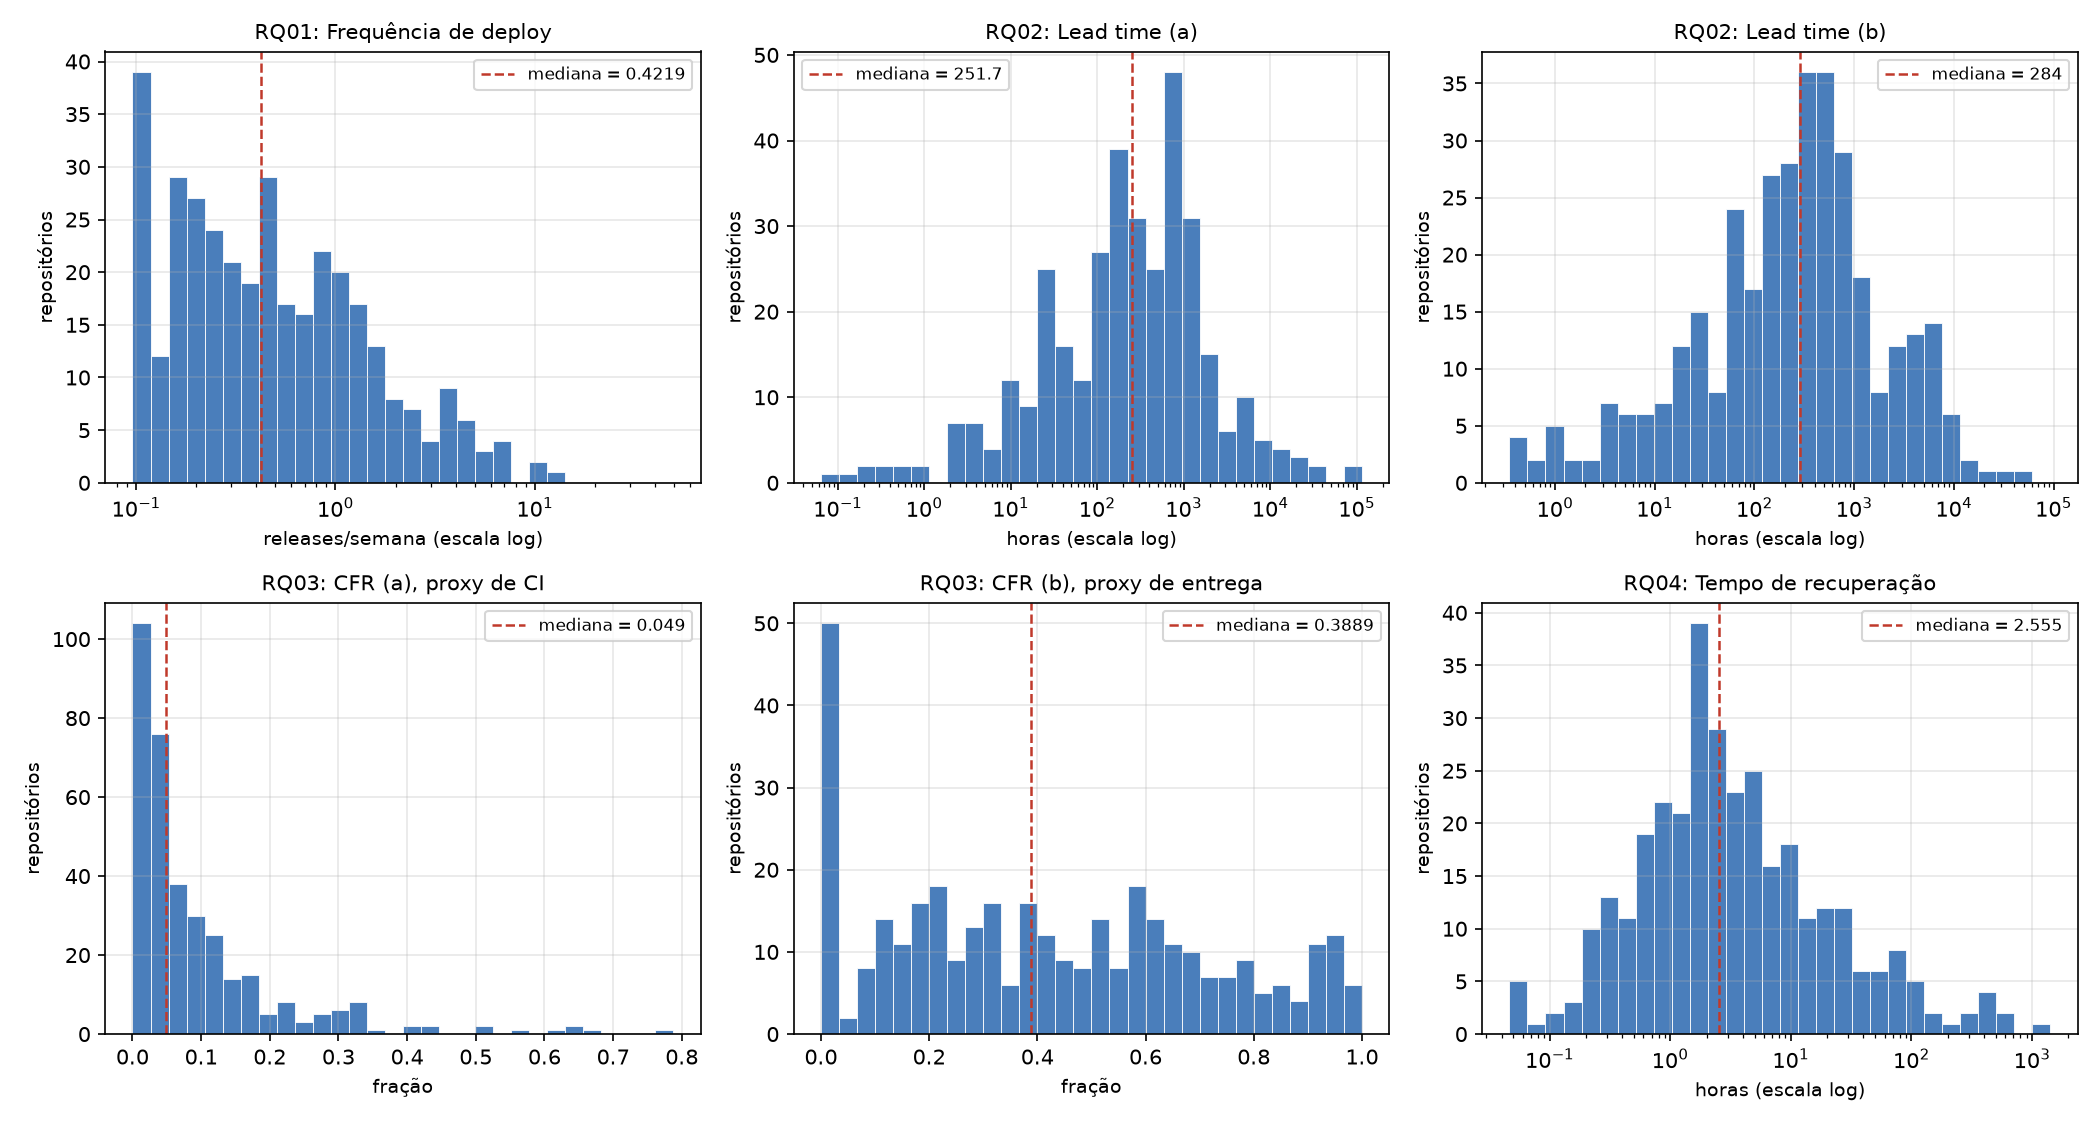
\includegraphics[width=0.92\textwidth]{rq1_rq4_distribuicoes.png}
\caption{Distribuição das seis métricas. Frequência, \textit{lead time} e recuperação em escala
logarítmica; a linha tracejada marca a mediana.}
\label{fig:distribuicoes}
\end{figure}

\textbf{RQ 01.} A mediana é de 0,42 \textit{release} por semana, cerca de uma a cada duas
semanas e meia. 260 repositórios (74,3\%) publicam menos de uma por semana, e só 5 (1,4\%)
alcançam o patamar \textit{Elite} de sete ou mais; 107 (30,6\%) ficam em \textit{Low} e 153
(43,7\%) em \textit{Medium}.

\textbf{RQ 02.} As variantes ficaram próximas: 251,7~h (10,5 dias) na (a) e 284,0~h (11,8
dias) na (b), com ICs quase sobrepostos e correlação de Spearman de 0,744 entre elas. Elas
divergem em repositórios específicos por construção: a variante (a) usa o \textit{commit}
mais antigo de cada \textit{release}, então um único \textit{commit} antigo ``esquecido'' num
ramo faz o \textit{lead time} daquela \textit{release} explodir, enquanto na (b) ele é só um
valor entre muitos e quase não move a mediana. Nas medianas da amostra as duas ficaram
próximas, mas o efeito aparece na cauda: o máximo é de $1{,}1 \times 10^{5}$~h na variante (a)
e de $9{,}3 \times 10^{4}$~h na (b). Pelos cortes
DORA, 57 repositórios ficam em \textit{Elite}, 89 em \textit{High}, 103 em \textit{Medium} e
101 em \textit{Low}.

\textbf{RQ 03.} A mediana do CFR (a) é 0,049 (IQR 0,100), e 13 repositórios (3,7\%) não têm
nenhum \textit{run} com falha; pelos cortes, 283 (80,9\%) ficam em \textit{Elite}. A mediana
do CFR (b) é 0,200 (IQR 0,364), quatro vezes maior, com 80 repositórios (22,9\%) em zero. As
duas variantes ordenam os repositórios de forma muito diferente: a correlação de Spearman
entre elas é de 0,107 ($p = 0{,}045$), e o IC 95\% vai de praticamente zero ($-0{,}0001$) a 0,21.

\textbf{RQ 04.} A mediana é de 2,56~h (IQR 8,55~h) nos 330 repositórios com ao menos um
episódio de falha seguida de sucesso. 196 (59,4\%) ficam em \textit{High} (de 1~h a menos de um
dia), 86 (26,1\%) em \textit{Elite} e 48 (14,5\%) em 24~h ou mais; o máximo é de 1.418~h. Os
20 repositórios (5,7\%) sem nenhum episódio ficam fora da mediana; a maioria deles não teve
falha alguma, como o \texttt{arendst/Tasmota}, com 569 \textit{runs} válidos. A censura foi
desprezível: mediana 0, terceiro quartil 0,0033, e 70,9\% dos repositórios sem nenhum episódio
censurado.

\textbf{Classificação geral.} 25 repositórios (7,1\%) são \textit{Elite}, 143 (40,9\%)
\textit{High}, 159 (45,4\%) \textit{Medium} e 23 (6,6\%) \textit{Low}. A nota de CFR puxa a
categoria para cima (\textit{Elite} em 80,9\% dos casos) e a de frequência para baixo
(\textit{Low} ou \textit{Medium} em 74,3\%).


% Resultados -- RQ 05 e RQ 06 (parte do Arthur).
% Números de resultados/rq5_spearman.csv e resultados/rq6_testes.csv.

\subsection{RQ 05: frequência de deploy e taxa de falha}

Calculamos a correlação de Spearman entre a frequência de \textit{deploy} e o CFR,
separadamente para cada variante. Spearman trabalha com postos, o que é adequado às
distribuições assimétricas observadas e ao grande número de empates em zero no CFR (a).

\begin{table}[ht]
\centering
\caption{Correlação entre frequência de \textit{deploy} e CFR, por variante.}
\label{tab:rq5}
\begin{tabular}{lrrrl}
\hline
\textbf{Variante do CFR} & \textbf{n} & $\boldsymbol{\rho}$ & \textbf{p} & \textbf{Interpretação} \\
\hline
(a) proxy de CI      & 350 & 0,127 & 0,017   & fraca positiva \\
(b) proxy de entrega & 350 & 0,613 & $<$ 0,001 & forte positiva \\
\hline
\end{tabular}
\end{table}

As duas são estatisticamente significativas ao nível de 5\%, mas o coeficiente da variante (b)
é quase cinco vezes o da (a). Na variante (a), um $\rho$ de 0,127 explica menos de 2\% da variância
conjunta: na prática, frequência de publicação e falha de CI são independentes nesta amostra.
Na variante (b), o $\rho$ de 0,613 indica associação forte. A Figura~\ref{fig:rq5} mostra as
duas dispersões, com a frequência em escala logarítmica.

\begin{figure}[ht]
\centering
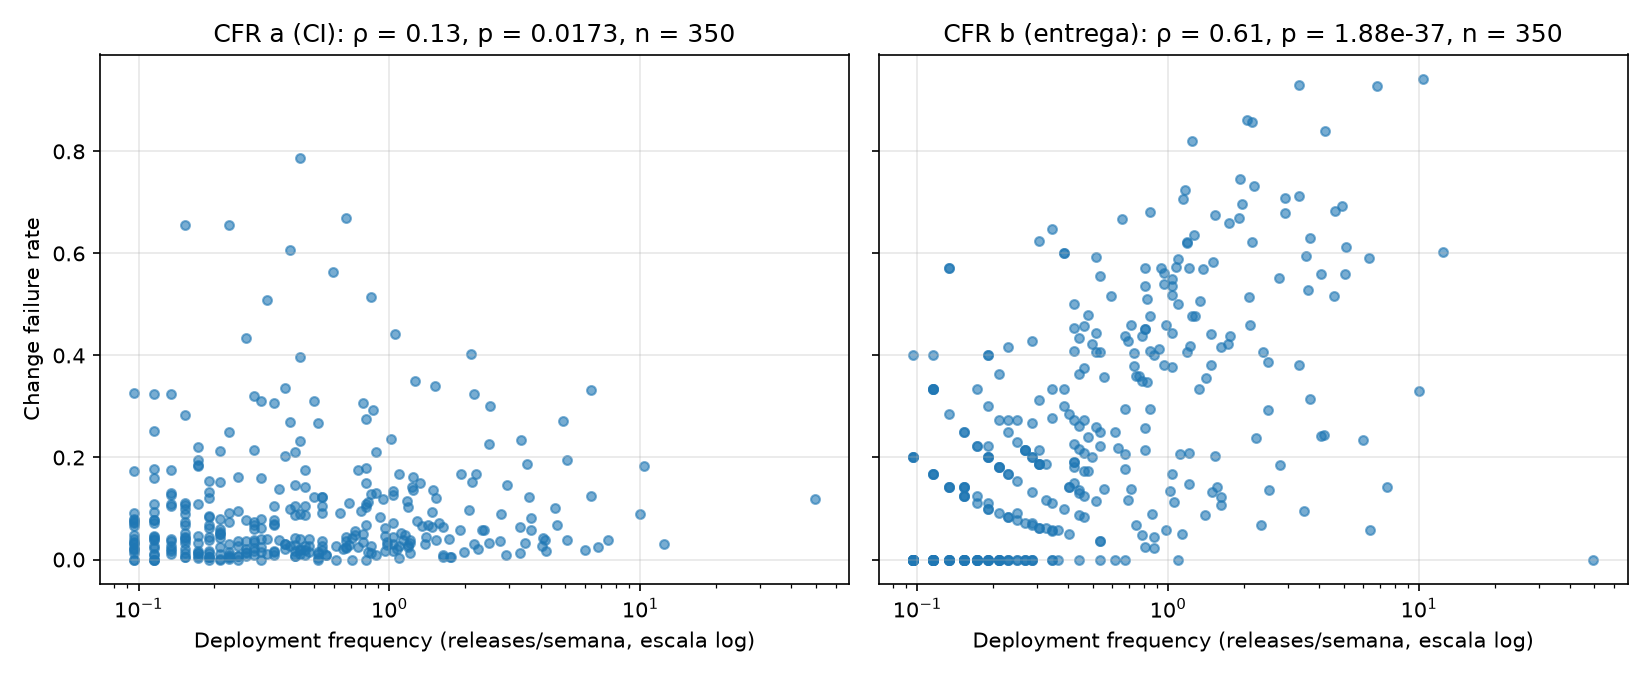
\includegraphics[width=\textwidth]{rq5_dispersao.png}
\caption{Frequência de \textit{deploy} (escala log) contra o CFR, nas duas variantes.}
\label{fig:rq5}
\end{figure}

\subsection{RQ 06: fatores associados ao desempenho}

Comparamos cada métrica entre subgrupos de cinco fatores: linguagem (as cinco mais frequentes,
e ``Outras''), quartis de estrelas, quartis de contribuidores, quartis de idade e tipo do
projeto. Usamos Kruskal-Wallis para três ou mais grupos e Mann-Whitney para dois, com
$\varepsilon^2$ e Cliff's delta como tamanho de efeito. Como são 30 testes simultâneos,
aplicamos a correção de Holm~\cite{holm1979} sobre o conjunto.

Doze dos 30 testes permanecem significativos após a correção (Tabela~\ref{tab:rq6}).

\begin{table}[ht]
\centering
\caption{Testes significativos após a correção de Holm, ordenados pelo tamanho de efeito.}
\label{tab:rq6}
\begin{tabular}{llrr}
\hline
\textbf{Fator} & \textbf{Métrica} & \textbf{p (Holm)} & $\boldsymbol{\varepsilon^2}$ \\
\hline
Idade          & Lead time (a) & $<$ 0,001 & 0,288 \\
Idade          & Lead time (b) & $<$ 0,001 & 0,251 \\
Contribuidores & Lead time (b) & $<$ 0,001 & 0,171 \\
Idade          & CFR (b)       & $<$ 0,001 & 0,164 \\
Idade          & Frequência    & $<$ 0,001 & 0,106 \\
Contribuidores & Lead time (a) & $<$ 0,001 & 0,104 \\
Linguagem      & Lead time (a) & $<$ 0,001 & 0,099 \\
Linguagem      & Frequência    & $<$ 0,001 & 0,097 \\
Linguagem      & CFR (b)       & $<$ 0,001 & 0,084 \\
Linguagem      & Lead time (b) & 0,001     & 0,078 \\
Idade          & Recuperação   & 0,016     & 0,051 \\
Estrelas       & Lead time (b) & 0,014     & 0,049 \\
\hline
\end{tabular}
\end{table}

Por fator, a idade aparece em cinco métricas, a linguagem em quatro, os contribuidores em
duas e as estrelas em uma. Nenhum teste sobre o tipo do projeto sobreviveu à
correção, e esse fator só existe para os 60 repositórios da amostra-ouro, de modo que os
testes sobre ele têm poder reduzido.

Entre os testes significativos, $\varepsilon^2$ vai de 0,049 a 0,288; o maior corresponde à
idade sobre o \textit{lead time} (a). Nenhum fator isolado explica a maior
parte da variação observada.

% Resultados -- RQ 07 e RQ 08 (parte do Pedro).
% Números de resultados/rq7_*.csv e resultados/rq8_*.csv.

\subsection{RQ 07: sensibilidade à definição de deploy}

Recalculamos a classificação DORA dos 350 repositórios sob três operacionalizações de
\textit{deploy}: \textbf{C1} (referência), que usa apenas \textit{releases}, com
\textit{lead time} (a) e CFR (a); \textbf{C2}, que inclui pré-\textit{releases} e adota as
variantes (b); e \textbf{C3}, que usa \textit{tags} com o CFR na variante (a).

\begin{table}[ht]
\centering
\caption{Distribuição das categorias DORA sob as três definições de \textit{deploy}.}
\label{tab:rq7dist}
\begin{tabular}{lrrr}
\hline
\textbf{Categoria} & \textbf{C1} & \textbf{C2} & \textbf{C3} \\
\hline
Elite  &  25 &   8 &  33 \\
High   & 143 & 134 & 164 \\
Medium & 159 & 186 & 138 \\
Low    &  23 &  22 &  15 \\
\hline
\end{tabular}
\end{table}

A concordância entre as classificações, medida pelo kappa ponderado, fica na faixa moderada
(Tabela~\ref{tab:rq7pares}). Entre um quarto e um terço dos repositórios trocam de categoria
conforme a definição adotada. A faixa \textit{Elite} é a mais sensível: vai de 8 repositórios
em C2 a 33 em C3, uma variação de quatro vezes sobre o mesmo conjunto de projetos e a mesma
janela de observação.

\begin{table}[ht]
\centering
\caption{Concordância entre as classificações, par a par.}
\label{tab:rq7pares}
\begin{tabular}{lrr}
\hline
\textbf{Par} & \textbf{Repositórios que mudam} & \textbf{Kappa ponderado} \\
\hline
C1 $\times$ C2 & 32,9\% & 0,515 \\
C1 $\times$ C3 & 25,4\% & 0,657 \\
C2 $\times$ C3 & 28,0\% & 0,602 \\
\hline
\end{tabular}
\end{table}

\subsection{RQ 08: rework rate}

O \textit{rework rate} é a proporção de \textit{releases} corretivas publicadas na janela,
calculada como \texttt{cfrb\_releases\_corretivas} dividido por \texttt{n\_releases}.
Diferente do CFR (b), ele conta toda \textit{release} corretiva, e não apenas as que vieram
em até 7 dias depois de outra.

\begin{table}[ht]
\centering
\caption{\textit{Rework rate} e CFR (b) nos 350 repositórios.}
\label{tab:rq8}
\begin{tabular}{lrrrr}
\hline
\textbf{Métrica} & \textbf{n} & \textbf{Q1} & \textbf{Mediana} & \textbf{Q3} \\
\hline
\textit{Rework rate} & 350 & 0,225 & 0,500 & 0,726 \\
CFR (b)              & 350 & 0,052 & 0,200 & 0,416 \\
\hline
\end{tabular}
\end{table}

A mediana do \textit{rework rate} é 2,5 vezes a do CFR (b). As duas medidas se correlacionam
($\rho = 0{,}522$, $p < 0{,}001$), mas \textbf{309 dos 350 repositórios têm \textit{rework
rate} maior que o CFR (b)}, e 21 não publicaram nenhuma \textit{release} corretiva na janela.

A leitura é direta: metade das \textit{releases} desses projetos corrige alguma coisa, mas
apenas uma em cada cinco corrige algo publicado na semana anterior. A maior parte do
retrabalho é manutenção de rotina, e não resposta a uma entrega recém-quebrada --- o que
reforça que o CFR (b), ao exigir a janela de 7 dias, mede um fenômeno mais estreito que
``\textit{release} corretiva''.


% ------------------------------------------------- Discussão e ameaças à validade
% Discussão e Ameaças à Validade (seções escritas pelos três).
% Números de resultados/, validacao/kappa.csv e dados/funil.csv.

\section{Discussão}

\textbf{As hipóteses sobre a taxa de falha erraram nas duas direções.} Esperávamos o CFR (a)
entre 10\% e 25\%, e ele ficou em 4,9\%. Os \textit{runs} contados são de \textit{push} no
\textit{default branch}, ou seja, de mudanças que já passaram por um \textit{pull request}
com CI; a métrica mede a falha do que já foi aprovado, que em projetos populares com revisão
obrigatória é baixa. Para o CFR (b) esperávamos valores iguais ou menores, e a mediana foi
quatro vezes maior. Parte disso vem do instrumento: a heurística adotada tem mais falsos
positivos (57) que falsos negativos (30) na amostra-ouro, então o valor de 0,200 tende a
superestimar o real. A única hipótese confirmada na RQ~03 foi a de que as variantes
concordariam pouco.

\textbf{As duas variantes do CFR medem coisas diferentes.} Com $\rho = 0{,}107$ e IC que
encosta no zero, um projeto bem avaliado por uma variante pode ser mal avaliado pela outra.
Recalculando a classificação geral com o CFR (b) no lugar do (a), 72 dos 350 repositórios
(20,6\%) mudam de categoria e a faixa \textit{Elite} cai de 25 para 8. No \textit{lead time} foi
diferente ($\rho = 0{,}744$ e medianas próximas), porque as duas variantes medem o mesmo evento
de formas diferentes, enquanto as do CFR medem eventos distintos: falha de \textit{pipeline}
antes da entrega e correção depois dela.

\textbf{A escala DORA e as releases open-source.} A frequência é a dimensão em que a amostra vai
pior, com 74,3\% dos repositórios abaixo de uma \textit{release} por semana. Isso diz mais sobre o
\textit{proxy} do que sobre a capacidade de entrega: uma \textit{release} é um marco de
versionamento, muitas vezes mensal ou trimestral, enquanto o \textit{deploy} do
DORA~\cite{dora2024} é a chegada de uma mudança à produção, e o patamar \textit{Elite} de sete por
semana pressupõe entrega contínua em ambiente corporativo~\cite{forsgren2018}. Como a categoria
geral é a mediana de quatro notas, ela acaba definida pelo par CFR (a) e recuperação, as
dimensões em que a amostra vai melhor.

\textbf{Velocidade e estabilidade (RQ 05).} As duas previsões se confirmaram na direção. Na
variante (a), a correlação é positiva mas fraca, e o IC exclui o zero por pouco: publicar com
mais frequência quase não vem acompanhado de mais falhas de CI, o que é compatível com a tese do
DORA de que velocidade e estabilidade não são um \textit{trade-off}. Na variante (b), a
correlação forte é em boa parte artefato da métrica, porque quem publica toda semana tem muito
mais chances de ter uma \textit{release} corretiva em até 7 dias do que quem publica a cada
trimestre. Com apenas a variante (b), a conclusão seria o oposto do que o DORA sustenta.

\textbf{O que explica as diferenças (RQ 06).} A idade é o fator mais associado ao desempenho:
projetos mais antigos acumulam mais tempo entre o \textit{commit} mais antigo e a publicação
($\varepsilon^2$ de 0,288 e 0,251 no \textit{lead time}) e publicam menos. A popularidade
quase não explica nada: o número de estrelas só aparece no \textit{lead time} (b), com o menor
efeito ($\varepsilon^2 = 0{,}049$).

\textbf{As conclusões são robustas? (RQ 07 e RQ 08).} Depende da RQ. A do \textit{lead time}
(RQ~02) se mantém nas duas variantes. As da taxa de falha (RQ~03 e 05) e a classificação geral
não se mantêm: trocar a variante do CFR muda a categoria de 20,6\% dos repositórios, e trocar a
unidade de \textit{deploy} muda entre 25\% e 33\%, e nenhum desses ICs desce abaixo de 21\%. O
\textit{rework rate} reforça a leitura do CFR (b): metade das \textit{releases} corrige algo, mas
só uma em cinco corrige algo publicado na semana anterior, então a maior parte da correção é
manutenção de rotina.

\section{Ameaças à Validade}

Seguimos as quatro categorias de Wohlin et al.~\cite{wohlin2012}.

\textbf{Construto.} \textit{Release} não é \textit{deploy}, e falha de CI não é falha em
produção: um \textit{run} que falha costuma ser um erro barrado antes de chegar ao usuário. A
validação manual sustentou o primeiro \textit{proxy} (as \textit{releases} representam entregas
reais em 59 dos 60 repositórios da amostra-ouro), mas a heurística de \textit{release} corretiva
não atingiu o F1 de 0,70 (0,65 na v4), e esse erro passa para o CFR (b), a RQ~08 e a C2 da
RQ~07. Os próprios avaliadores divergiram em 26 de 299 \textit{releases}. Rebase e
\textit{squash merge} reescrevem o \texttt{commit.author.date} e afetam o \textit{lead time}
em direção desconhecida.

\textbf{Interna.} As análises são correlacionais. A idade se correlaciona com a frequência
($\rho = -0{,}306$), assim como as estrelas ($\rho = 0{,}162$) e os contribuidores
($\rho = 0{,}119$), e esses fatores não são controlados nas RQ~01 a 04. O filtro de inclusão
(5 \textit{releases} e 50 \textit{runs}) deixa só projetos que já versionam e automatizam com
regularidade, e o descarte dos seis repositórios com mais de 1.000 \textit{runs} por dia tira
da amostra os de maior atividade de CI.

\textbf{Externa.} A amostra não é aleatória: entraram os 1.000 mais estrelados de cada faixa, e
os menos estrelados de cada faixa nunca foram observados. Os resultados valem para repositórios
populares com GitHub Actions, e não se transferem para equipes corporativas, que são o contexto
das faixas DORA. A janela é única, de 12 meses, e não separa característica estável de efeito
do período.

\textbf{Conclusão.} Usamos mediana, IQR e testes não paramétricos por causa da assimetria, e a
correção de Holm nos 30 testes da RQ~06. O tipo do projeto só existe para 60 repositórios, e os
testes sobre ele têm pouco poder. Os ICs por \textit{bootstrap} mostram que as medianas e as
proporções de mudança de categoria são estáveis, mas que a correlação entre as variantes do CFR
não se distingue com segurança de zero.


% ---------------------------------------------------------------- Conclusão
\section{Conclusão}

Medimos as quatro métricas DORA em 350 repositórios \textit{open-source} populares usando
somente dados públicos do GitHub. A amostra publica pouco (mediana de 0,42 \textit{release} por
semana), leva cerca de dez dias entre o \textit{commit} mais antigo e a publicação, falha pouco
no CI (mediana de 0,049) e se recupera rápido (mediana de 2,56~h); 86,3\% dos repositórios são
\textit{High} ou \textit{Medium}.

Esses valores dependem bastante de decisões de medição. As duas variantes da taxa de falha
correlacionam-se a $\rho = 0{,}107$ e discordam sobre a categoria de 20,6\% da amostra; trocar
a definição de \textit{deploy} move entre 25\% e 33\% dos repositórios, e a faixa
\textit{Elite} varia de 8 a 33 projetos. Na validação manual, o \textit{proxy} de \textit{release} se sustentou (59 de 60
repositórios), mas a melhor heurística de \textit{release} corretiva ficou em F1 de 0,65, numa
dimensão em que os próprios avaliadores divergiram em 26 de 299 casos. Uma classificação DORA
de projetos \textit{open-source} só pode ser interpretada junto com as escolhas operacionais
que a produziram.

Como trabalhos futuros, sugerimos usar projetos com ambiente de produção observável no lugar
do \textit{proxy} de \textit{release}, estender a janela para além de 12 meses e ampliar a
amostra-ouro para treinar e validar a heurística em conjuntos disjuntos.

\section*{Disponibilidade dos dados}

Código, dados e roteiros de análise: \url{https://github.com/candian15/LabExpGRP} (pasta
\texttt{LAB03}). Quadro do GitHub Projects:
\url{https://github.com/users/candian15/projects/2}.

\bibliographystyle{sbc}
\bibliography{referencias}

\end{document}
